\subsection{Tune the IMM-PDAF to the Given Simulated Data}

We initialized the filter using the values from previous exercises which we knew worked well. We then modified the \textit{simulate\_atc\_track.m} script to allow us to generate pure CV and CT tracks and used those to tune the corresponding CV/CT PDAF models, using the NEES $95 \%$ confidence interval (CI) and common sense as metrics. Multiple simulated tracks were used for each model to increase robustness. The measurement noise $r$, clutter intensity $\lambda$, the detection probability $P_D$ and the gate size should be independent of modes, so they were tuned and balanced between the two models. The clutter rate $\lambda$ can be interpreted as the number of false detections per cubic meter and it is therefore reasonable for this number to be quite low. The process noise for CV $q_{cv}$ and CT $q_{ct}$ were tuned individually using their correspondig models. For IMM PDAF tuning we created a custom plot function which allowed us to plot the tracked path in colors corresponding to the mode probability (see \cref{fig:task22_modeprob}). We then tuned the IMM Markov Matrix $\pi$ so that the CV model was used during constant velocity sections of the track, and the CT models during the turns (fig \ref{fig:task22_modeprob_tuned}). $q_{cv}$ and $q_{ct}$ does affect the mode probabilities, i.e we risk always preferring one model if the process noises are not balanced (see fig \ref{fig:task22_modeprob_highcv} where $q_{cv}$ is big compared to $q_{ct}$). Our finished tuning works well and seems to balance the two models well. The NEES is mostly within the $95\%$ CI as can be seen in \cref{fig:task22_NEES}. The estimation error, as shown in \cref{fig:task22_tracking_error}, is also quite small and well within what we consider acceptable limits.

\begin{tcolorbox}[ams align, title={Tuning for IMM-PDAF in simulated dataset}]
        r &= 5 & \lambda &= 10^{-4} \label{eq:imm-sim-tuning1} \\
        P_D &= 0.95 & \texttt{gateSize} &= 5^2 \label{eq:imm-sim-tuning2} \\
        q_{cv} &= 0.0078  & q_{ct} &= \begin{bmatrix}0.02 & 0.0005\end{bmatrix} \label{eq:imm-sim-tuning3} \\
        \Pi &= \begin{bmatrix}0.90 & 0.05 \\ 0.10 & 0.95\end{bmatrix} \label{eq:imm-sim-tuning4}
\end{tcolorbox}

\begin{figure}
    \centering
    \hspace*{-2cm}\begin{adjustbox}{minipage=0.8\linewidth, scale=1}
        \begin{subfigure}{.5\textwidth}
            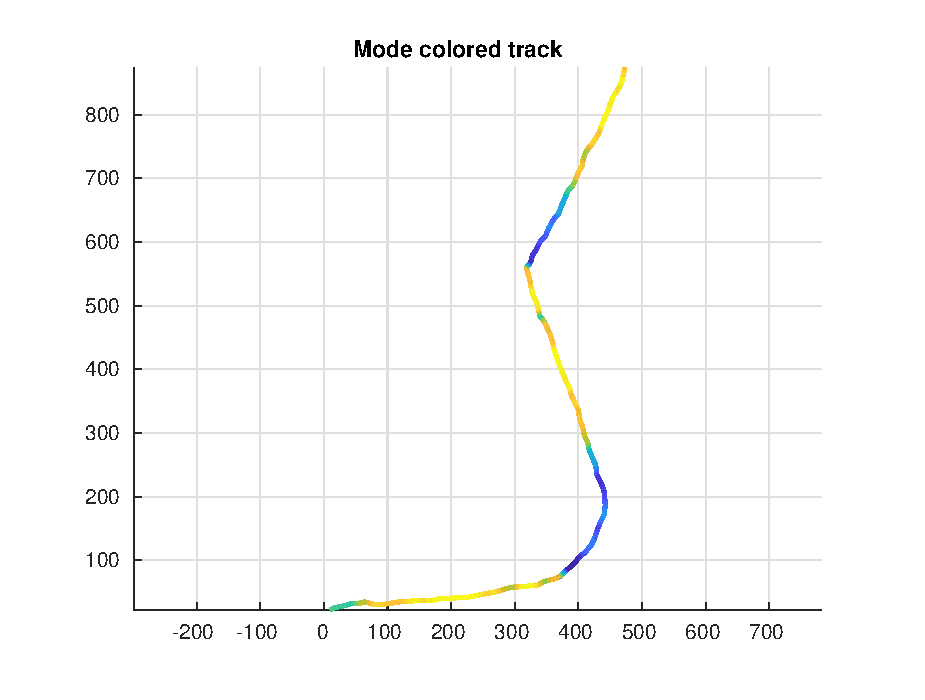
\includegraphics[width=\linewidth]{plots/task22_modeprob.eps}
            \caption{Our tuning}
            \label{fig:task22_modeprob_tuned}
        \end{subfigure}
        \begin{subfigure}{.5\textwidth}
            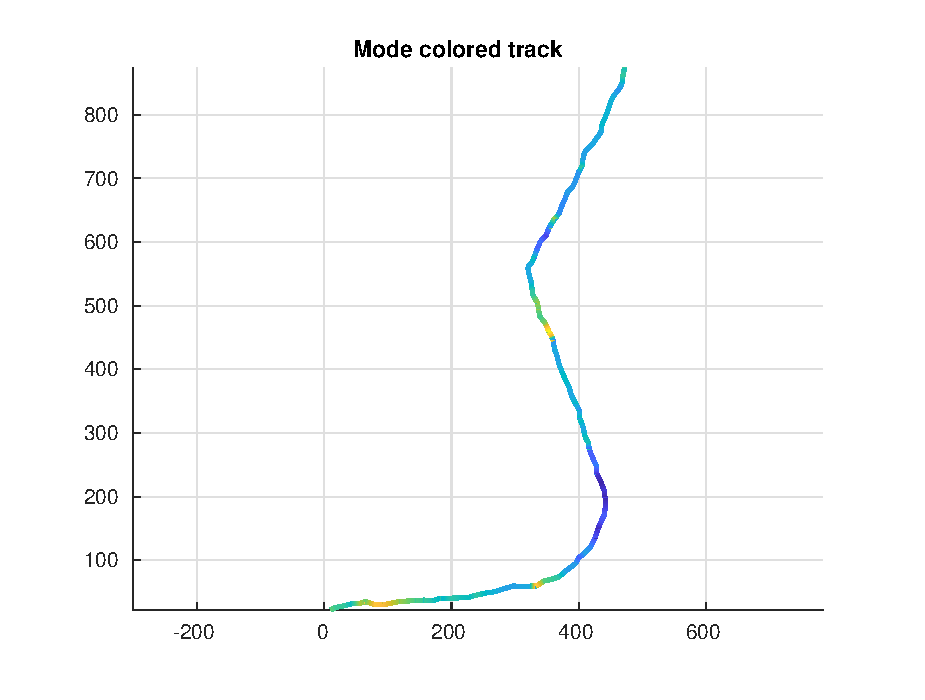
\includegraphics[width=\linewidth]{plots/task22_modeprob_highcv.eps}
            \caption{$q_{cv}$ and $q_{ct}$ not in balance}
            \label{fig:task22_modeprob_highcv}
        \end{subfigure}
    \end{adjustbox}
        \caption{Mode probability plot: Yellow = CV, Blue = CT}
        \label{fig:task22_modeprob}
\end{figure}

\begin{figure}
    \centering
    \hspace*{-2cm}\begin{adjustbox}{minipage=0.8\linewidth, scale=1}
        \begin{subfigure}{.5\textwidth}
            \includegraphics[width=\linewidth]{plots/a1/task2/a1_task2_error.eps}
            \caption{Tracking error}
            \label{fig:task22_tracking_error}
        \end{subfigure}
        \begin{subfigure}{.5\textwidth}
            \includegraphics[width=\linewidth]{plots/a1/task2/a1_task2_NEES.eps}
            \caption{NEES}
            \label{fig:task22_NEES}
        \end{subfigure}
    \end{adjustbox}
        \caption{Tracking performance when using simulated data}
\end{figure}
